\documentclass[12pt, letterpaper]{article}
\usepackage[utf8]{inputenc}
\usepackage{amsmath, amssymb, amsthm}
\usepackage{mathtools}

\usepackage{fancyhdr}
\usepackage{lipsum} % For placeholder text, you can remove this in your actual document.

\usepackage[headings]{fullpage} % Set margins and place page numbers at bottom center
\usepackage[shortlabels]{enumitem} % Use a. in the enumerate
\usepackage{amsmath} % aligned equations
\usepackage{graphicx} % include figure
\usepackage{float} % usage of H for figure float
\usepackage{amssymb} % \blacksqure
\usepackage{xhfill} % fill horizontal line
\usepackage{xcolor} % colors
\usepackage{sectsty} % section coloring
\subsectionfont{\color{blue}}  % sets colour of sections

\pagestyle{fancy}
\fancyhf{} % Clear header and footer fields
\renewcommand{\headrulewidth}{0.4pt} % Horizontal line under the header
\setlength{\headheight}{18pt}

\fancyhead[L]{\large MATH 551-001 \scriptsize Fall 2023}
\fancyhead[C]{}
\fancyhead[R]{\large \textbf{Ali Zafari - 800350381}} % Page number on the right side
\fancyfoot[R]{\thepage}

\newcommand{\Z}{\mathbb{Z}}
\newcommand{\R}{\mathbb{R}}
\newcommand{\C}{\mathbb{C}}
\newcommand{\F}{\mathbb{F}}
\newcommand{\bigO}{\mathcal{O}}
\newcommand{\Real}{\mathcal{Re}}
\newcommand{\poly}{\mathcal{P}}
\newcommand{\mat}{\mathcal{M}}
\renewcommand{\L}{L}
\newcommand{\U}{U}
\DeclareMathOperator{\Span}{span}
\newcommand{\Hom}{\mathcal{L}}
\DeclareMathOperator{\Null}{null}
\DeclareMathOperator{\Range}{range}
\newcommand{\defeq}{\vcentcolon=}
\newcommand{\restr}[1]{|_{#1}}
\renewcommand{\inf}{\mathop{\mathrm{inf}\vphantom{\mathrm{sup}}}}

\begin{document}

\subsection*{1\hspace{1pt}A\hspace{20pt}Exercise 12 }
Since $f$ is Riemann integrable, for $\epsilon>0$ there exists partition $P=\{x_0, x_1,\dots,x_n\}$ on $[a, b]$ such that $\U(f, P, [a,b])-\L(f, P, [a,b])<\epsilon$ (using Theorem ($\spadesuit$) proven below).
\\\\
Using reverse triangular inequality, $\forall x,y\in[x_{i-1}, x_i]$ where $i\in\{1,2,\dots,n\}$:
\begin{align*}
    \Bigl||f(x)|-|f(y)|\Bigr|
    &\leq
    \Bigl|f(x)-f(y)\Bigr|\\
    \sup_{x,y\in[x_{i-1}, x_i]}\Bigl||f(x)|-|f(y)|\Bigr|
    &\leq
    \sup_{x,y\in[x_{i-1}, x_i]}\Bigl|f(x)-f(y)\Bigr|\\
    \sup_{[x_{i-1}, x_i]}|f|-\inf_{[x_{i-1}, x_i]}|f|
    &\leq
    \sup_{[x_{i-1}, x_i]}f-\inf_{[x_{i-1}, x_i]}f \qquad\tag{$*$}
\end{align*}
where last line follows from Lemma ($\clubsuit$) proven below.
\\\\
Now we have
\begin{align*}
    \U(|f|, P, [a,b])-\L(|f|, P, [a,b])
    &=
    \sum_{i=1}^n(x_i-x_{i-1})(\sup_{[x_{i-1}, x_i]}|f|-\inf_{[x_{i-1}, x_i]}|f|)\\
    &\leq
    \sum_{i=1}^n(x_i-x_{i-1})(\sup_{[x_{i-1}, x_i]}f-\inf_{[x_{i-1}, x_i]}f)\qquad \qquad\text{using $(*)$}\\
    &=
    \U(f, P, [a,b])-\L(f, P, [a,b])< \epsilon\qquad \qquad\text{Theorem ($\spadesuit$)}
\end{align*}
\\
therefore
\begin{align*}
    \U(|f|, P, [a,b])-\L(|f|, P, [a,b]) < \epsilon
\end{align*}
and again according to Theorem ($\spadesuit$), $|f|$ is Riemann integrable.
\\\\
In addition, since $-|f|\leq f\leq|f|$ and all $f$, $|f|$ and $-|f|$ are Riemann integrable,
\begin{align*}
    -\int_a^b|f|\leq\int_a^bf\leq\int_a^b|f|\quad\Longrightarrow\quad\left|\int_a^bf\right|\leq\int_a^b|f|
\end{align*}
\hrule

\subsubsection*{Lemma ($\clubsuit$)}
{\color{violet}Suppose $g: [a,b]\rightarrow \R$ is a bounded function. Let $P=\{x_0, x_1, . . . , x_n\}$ be a partition of
$[a, b]$. Then for each $i\in \{1, 2,\dots, n\}$,
\begin{align*}
    \sup_{[x_{i-1}, x_i]}g-\inf_{[x_{i-1}, x_i]}g=\sup_{x,y\in[x_{i-1}, x_i]}\Bigl|g(x)-g(y)\Bigr|
\end{align*}
}\textbf{proof.}
\begin{itemize}
    \item Let $x,y\in[x_{i-1}, x_i]$ and WLOG $g(x)\geq g(y)$. Therefore $\sup_{[x_{i-1}, x_i]}g\geq g(x)$ and $\inf_{[x_{i-1}, x_i]}g\leq g(y)$, as a result
    \begin{align*}
        \sup_{[x_{i-1}, x_i]}g-\inf_{[x_{i-1}, x_i]}g
        &\geq
        g(x)-g(y)\\
        \sup_{[x_{i-1}, x_i]}g-\inf_{[x_{i-1}, x_i]}g
        &\geq
        |g(x)-g(y)|\qquad\qquad(g(x)\geq g(y))\\
        \sup_{[x_{i-1}, x_i]}g-\inf_{[x_{i-1}, x_i]}g
        &\geq
        \sup_{x,y\in[x_{i-1}, x_i]}|g(x)-g(y)| \tag{1}
    \end{align*}
    \item let $\epsilon>0$. $\exists x,y\in[x_{i-1}, x_i]$ such that $g(x)>\sup_{[x_{i-1}, x_i]}g-\frac{\epsilon}{2}$ and $g(y)<\inf_{[x_{i-1}, x_i]}g+\frac{\epsilon}{2}$. Therefore $g(x)-g(y)>\sup_{[x_{i-1}, x_i]}g-\inf_{[x_{i-1}, x_i]}g-\epsilon$. Then equivalently $|g(x)-g(y)|>\sup_{[x_{i-1}, x_i]}g-\inf_{[x_{i-1}, x_i]}g-\epsilon$:
    \begin{align*}
        \sup_{x,y\in[x_{i-1}, x_i]}|g(x)-g(y)|
        &>
        \sup_{[x_{i-1}, x_i]}g-\inf_{[x_{i-1}, x_i]}g-\epsilon \qquad\qquad \forall\epsilon>0\\
        \sup_{x,y\in[x_{i-1}, x_i]}|g(x)-g(y)|
        &\geq
        \sup_{[x_{i-1}, x_i]}g-\inf_{[x_{i-1}, x_i]}g\tag{2}
    \end{align*}
\end{itemize}
By having (1) and (2), the equality holds true.\\
\hrule
\subsubsection*{Theorem ($\spadesuit$) \qquad [1\hspace{1pt}A\hspace{5pt}Exercise 3]}
{{\color{violet}Suppose $f: [a,b]\rightarrow \R$ is a bounded function. $f$ is Riemann integrable if and only if for each $\epsilon>0$, there exists a partition $P$ of $[a,b]$ such that 
\begin{align*}
    \U(f, P, [a,b])-\L(f, P, [a,b])<\epsilon
\end{align*}
}\textbf{proof.}
\begin{itemize}[label={}]
    \item``$\Leftarrow$"
        Suppose the condition holds. Let $\epsilon>0$ and choose a partition $P$ which satisfies the condition. Since $U(f,[a,b])\leq U(f,P,[a,b])$ and $L(f,[a,b])\geq L(f,P,[a,b])$
        \begin{align*}
            0\leq U(f,[a,b])-L(f,[a,b])\leq U(f,P,[a,b])-L(f,P,[a,b])<\epsilon
        \end{align*}
        since $\epsilon$ is chosen arbitrarily, $U(f,[a,b])-L(f,[a,b])=0$ and $f$ is Riemann integrable.
    \item``$\Rightarrow$"
        Suppose $f$ is Riemann integrable. Given $\epsilon>0$, $\exists$ partitions $Q,R$ such that $U(f,Q,[a,b])<U(f,[a,b]) +\frac{\epsilon}{2}$ and $L(f,R,[a,b])>L(f,[a,b])-\frac{\epsilon}{2}$. Let P be a common refinement of $Q$ and $R$, then
        \begin{align*}
            U(f,P,[a,b])-L(f,P,[a,b])\leq U(f,Q,[a,b])-L(f,R,[a,b])<\underbrace{U(f,[a,b])-L(f,[a,b])}_{=0}+\epsilon\\
        \end{align*}
        therefore $U(f,P,[a,b])-L(f,P,[a,b])<\epsilon$.
\end{itemize}

\clearpage

\subsection*{1\hspace{1pt}A\hspace{20pt}Exercise 13}
Let $\epsilon>0$. Assume equidistant partition $P_\epsilon=\{x_0, x_1, \dots, x_n\}$ defined on $[a,b]$ such that $x_i-x_{i-1}=x_j-x_{j-1}<\frac{\epsilon}{f(b)-f(a)}\quad \forall i,j\in\{1,\dots,n\}$, then
\begin{align*}
    \U(f, P_\epsilon, [a,b])-\L(f, P_\epsilon, [a,b])&=\sum_{i=1}^n(x_i-x_{i-1})(\sup_{[x_{i-1}, x_i]}f-\inf_{[x_{i-1}, x_i]}f)\\
    &=(x_i-x_{i-1})\sum_{i=1}^n\sup_{[x_{i-1}, x_i]}f-\inf_{[x_{i-1}, x_i]}f\\
    &=(x_i-x_{i-1})\sum_{i=1}^nf(x_i)-f(x_{i-1})\qquad \text{($f$ increasing)}\\
    &=(x_i-x_{i-1})(f(b)-f(a))\\
    &< \frac{\epsilon}{f(b)-f(a)}(f(b)-f(a))=\epsilon
\end{align*}
therefore according to Theorem ($\spadesuit$) stated below, f is Riemann integrable.\\

\hrule

\subsubsection*{Theorem ($\spadesuit$)}
{\color{violet}Suppose $f: [a,b]\rightarrow \R$ is a bounded function. $f$ is Riemann integrable if and only if for each $\epsilon>0$, there exists a partition $P$ of $[a,b]$ such that 
\begin{align*}
    \U(f, P, [a,b])-\L(f, P, [a,b])<\epsilon
\end{align*}
}\textbf{proof.} Proven as part of the solution for {\color{blue}1A Exercise 12}.
\clearpage

\subsection*{1\hspace{1pt}B\hspace{20pt}Exercise 1}
Since set of irrational numbers is dense, no matter of how we choose a partition $P$ on $[0,1]$, an irrational number exists in $[x_{i-1},x_i]$, therefore $\inf_{[x_{i-1}, x_i]}f=0$ and then $L(f,P,[0,1])=0$.
\\\\
According to Theorem ($\spadesuit$) stated below, if we show $U(f,P,[a,b])<\epsilon$ for arbitrary choice of $\epsilon$, then $f$ will be Riemann integrable.
\\
Let $A_n=\{x: f(x)\geq \frac{1}{n}\}$ then for any $x=\frac{i}{j}\in A_n$, $i,j\leq n$. Therefore $A_n$ is a finite set ($|A_n|<\infty$).
\\
Let $\epsilon>0$. Then assume $\frac{1}{n}<\frac{\epsilon}{2}$. We choose $P$ such that each member of $A_n$ falls into $[x_{i-1}, x_i]$ by having
\begin{align*}
    x_i-x_{i-1}<\frac{\epsilon}{2|A_n|}
\end{align*}
Let $B:=\{i: A_n\cap[x_{i-1}, x_i]=\emptyset\}$ so $|B|<|A_n|$.
\begin{itemize}
    \item if $i\in B$ then $\sup_{[x_{i-1}, x_i]}f<\frac{1}{n}<\frac{\epsilon}{2}$
    \item if $i\notin B$ then $\sup_{[x_{i-1}, x_i]}f=1$
\end{itemize}
then we have
\begin{align*}
    U(f,P,[a,b])
    &=
    \sum_{i\in B}(x_i-x_{i-1})\sup_{[x_{i-1}, x_i]}f+\sum_{i\notin B}(x_i-x_{i-1})\sup_{[x_{i-1}, x_i]}f\\
    &<
    \sum_{i\in B}(x_i-x_{i-1})\frac{\epsilon}{2}+\sum_{i\notin B}(x_i-x_{i-1})(1)\\
    &<
    \frac{\epsilon}{2}+|A_n|\frac{\epsilon}{2|A_n|}=\epsilon
\end{align*}
therefore $f$ is Riemann integrable and $\int_0^1f=0$.\\
\hrule

\subsubsection*{Theorem ($\spadesuit$)}
{\color{violet}Suppose $f: [a,b]\rightarrow \R$ is a bounded function. $f$ is Riemann integrable if and only if for each $\epsilon>0$, there exists a partition $P$ of $[a,b]$ such that 
\begin{align*}
    \U(f, P, [a,b])-\L(f, P, [a,b])<\epsilon
\end{align*}
}\textbf{proof.} Proven as part of the solution for {\color{blue}1A Exercise 12}.
\clearpage

\subsection*{1\hspace{1pt}B\hspace{20pt}Exercise 5}
Let continuous $f_n$ be defined as
\begin{align*}
    f_n(x)=
    \begin{cases} 
      4n^2x & 0\leq x\leq \frac{1}{2n} \\
      4n-4n^2x & \frac{1}{2n} < x\leq \frac{1}{n} \\
      0 &\frac{1}{n} < x \leq 1
   \end{cases}
\end{align*}
as shown in Figure \ref{fig:tent}.
\begin{figure}[h]
    \centering
    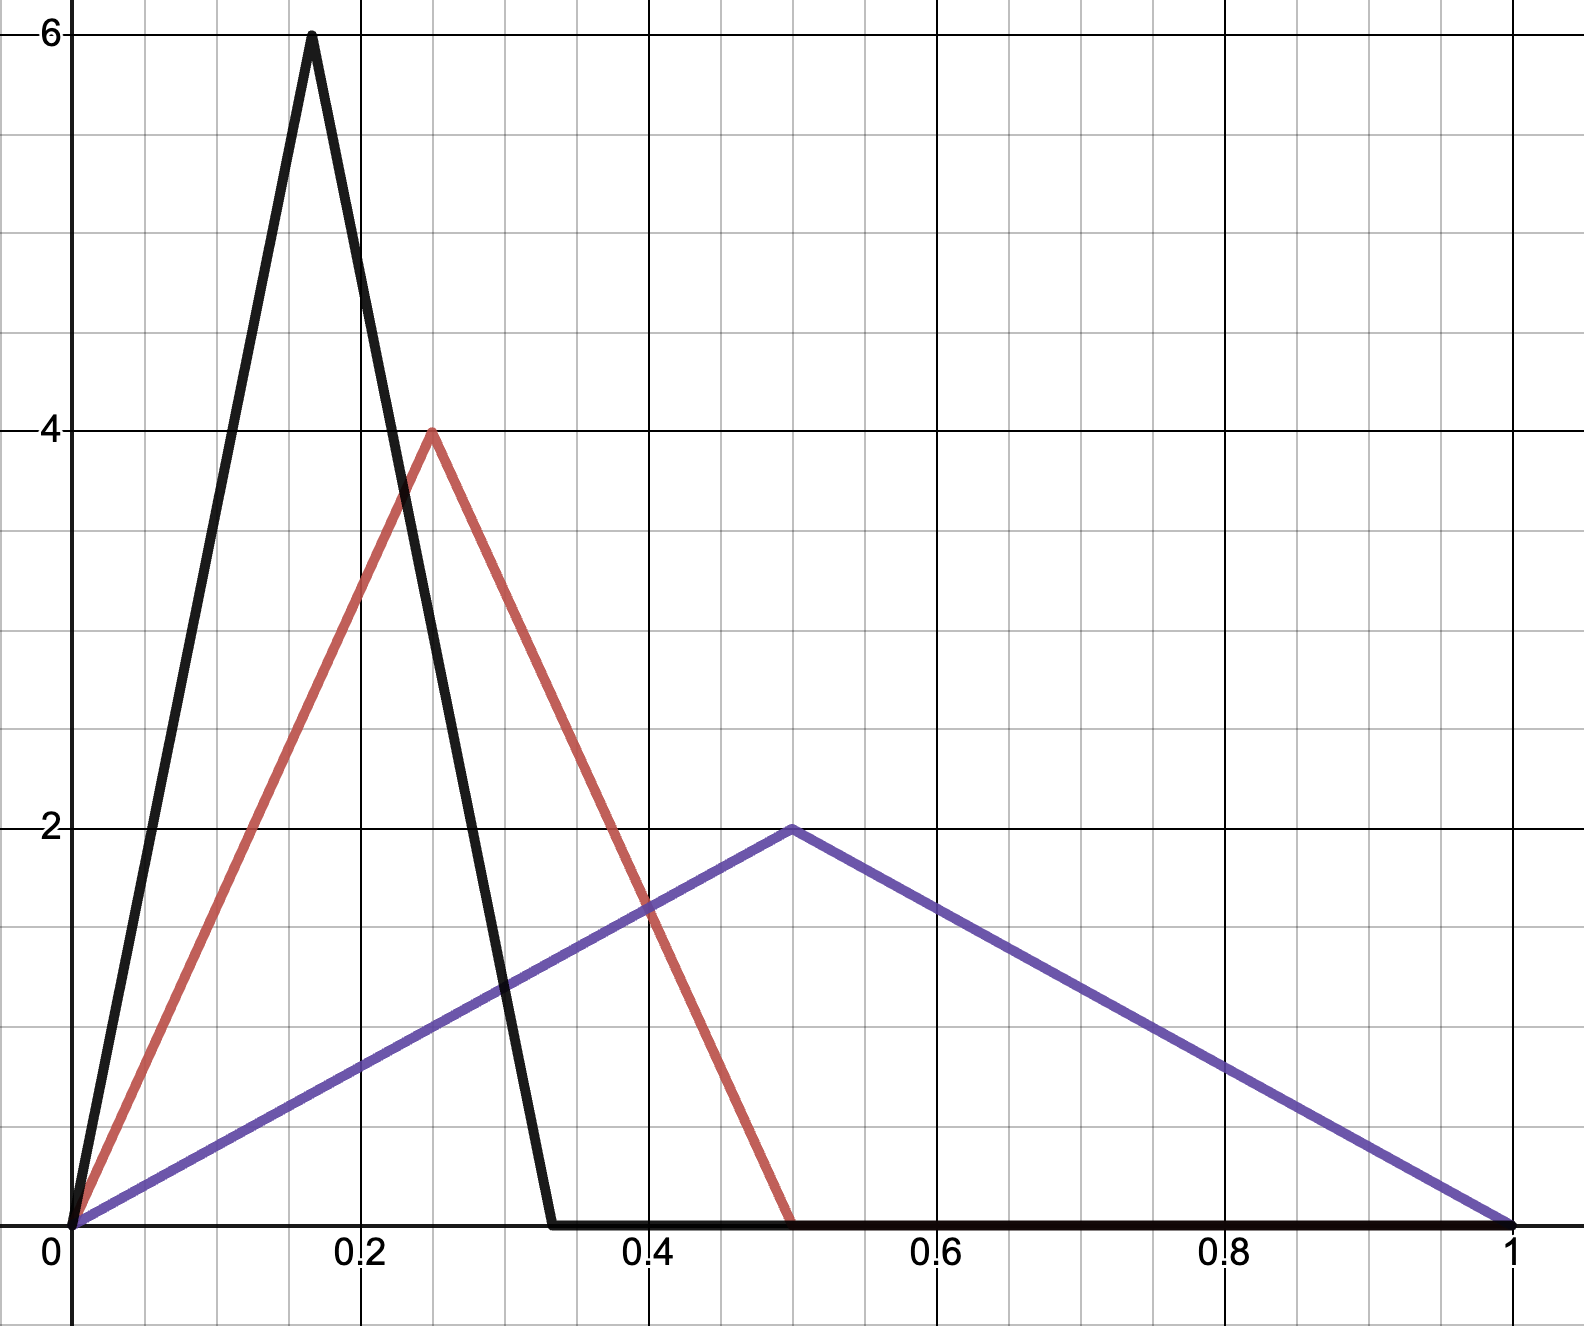
\includegraphics[width=0.5\textwidth]{figures/HW1/tent.png}
    \caption{Function $f_n$ defined on $[0,1]$ plotted for $n=1,2,3$.}
    \label{fig:tent}
\end{figure}

Also we have
\begin{align*}
    f(x)=\lim_{n\longrightarrow\infty}f_n(x)=0 \quad 0\leq x\leq 1
\end{align*}
Now for integral of each $f_n$ we have
\begin{align*}
    \lim_{n\longrightarrow\infty}\int_0^1f_n=\lim_{n\longrightarrow\infty}1=1
\end{align*}
while for the integral of limit of $f_n$ 
\begin{align*}
    \int_0^1f=\int_0^1\lim_{n\longrightarrow\infty}f_n=\int_0^10=0
\end{align*}
Therefore
\begin{align*}
   \int_0^1f\neq\lim_{n\longrightarrow\infty}\int_0^1f_n
\end{align*}
for this choice of $f_n$.
\clearpage

\end{document}
